%
%
%If you would like a word document version of the case study, email mchester@es.net.
%
%Last revised: March 6, 2015 by Mary Hester.
%
%Note: document should be built using  XeLaTeX.

\documentclass[10pt,a4paper]{report}

\usepackage{geometry}       
\usepackage{amsfonts}
\usepackage{kpfonts}
\usepackage[parfill]{parskip}
\usepackage{graphicx}
\usepackage{amssymb}
\usepackage{fullpage}
\usepackage{caption}
\usepackage{tabulary}

\usepackage{array}
\usepackage{xcolor,colortbl}
\usepackage{booktabs}

\usepackage{graphicx}
\usepackage{caption}
\usepackage{subcaption}
\usepackage{wrapfig}

%%Reset font for Helvetic. Needs to be built using XeLatex
\usepackage{fontspec,xltxtra,xunicode}
\defaultfontfeatures{Mapping=tex-text}
\setromanfont[Mapping=tex-text]{Helvetica}
\setsansfont[Scale=MatchLowercase,Mapping=tex-text]{Helvetica}
\setmonofont[Scale=MatchLowercase]{Helvetica}

%renaming default "Chapter" headings
\renewcommand{\chaptername}{Case Study}

\begin{document}

\chapter{KBase - DOE Systems Biology KnowledgeBase}

\section{Background} 
%From a networking and data perspective, describe the science research and/or details of your facility (if applicable), or the focus of your current projects. (1-2 paragraphs total.)
The Department of Energy Systems Biology Knowledgebase (KBase) is a software and data platform designed to meet the grand challenge of systems biology: predicting and designing biological function. KBase integrates data, tools, and their associated interfaces into one unified, scalable environment, so users do not need to access them from numerous sources or learn multiple systems in order to perform sophisticated systems biology analyses. Users can perform large-scale analyses and combine multiple lines of evidence to model plant and microbial physiology and community dynamics.  KBase is the first large-scale bioinformatics system that enables users to upload their own data, analyze it (along with collaborator and public data), build increasingly realistic models, and share and publish their workflows and conclusions. KBase aims to provide a knowledgebase: an integrated environment where knowledge and insights are created and multiplied.

Underlying the KBase platform is a service-oriented architecture that runs across a distributed set of resources located at Argonne National Lab and Lawrence Berkeley National Lab.  The two sites mirror one another both in data and services.  KBase takes advantages of existing connectivity to ESnet at both sites.  KBase uses its connectivity to 1) replicate data between the two sites 2) enable users to upload/download data into the KBase system.

\section{Network and Data Architecture}
%Please describe the network architecture for your facility and/or laboratory and/or campus.  It is critical for us to know how your data moves from your location on campus, to the campus network, and then to the broader Internet.  Details should include local infrastructure configuration, bandwidth speed(s), hardware, etc. Any specific items of interest in regard to high-performance data transfers, network architecture (e.g., a Science DMZ http://fasterdata.es.net/science-dmz/) or other site, campus, or facility networking issues? Please include network diagrams if possible.

KBase is connected to ESnet directly at the two major sites (Argonne National Lab and Lawrence Berkeley National Lab).  Both sites are effectively connected at 10Gb, but the way in which the connect to ESnet is slightly different at the two sites.

At Berkeley, KBase is housed with NERSC.  This is currently at the Oakland Scientific Facility but will move in late 2015 to the new Computational Research and Theory (CRT) Facility which has just completed construction.  Currently a dedicated KBase router (Juniper QFX3500S) is connected via 10Gb to a NERSC owned Alcatel-based 100Gb router which is connected to ESnet via a 100Gb link.  The connection through the NERSC router is VLAN based (i.e. the NERSC router doesn't perform any Layer 3 routing).  KBase servers are connected to the Juniper via a Mellanox 40Gb Ethernet Switch.  Currently, the Juniper router has a minimal set of ACLs defined.  The Juniper QFX3500s has four 40Gb interfaces which are not currently being used, but could be used to increase the bandwidth in the future.

At Argonne, KBase is co-located with the Magellan cloud and shares network connectivity.  Figure \ref{kbase:anl} illustrates this connectivity.

\begin{figure}[htbp]
\begin{center}
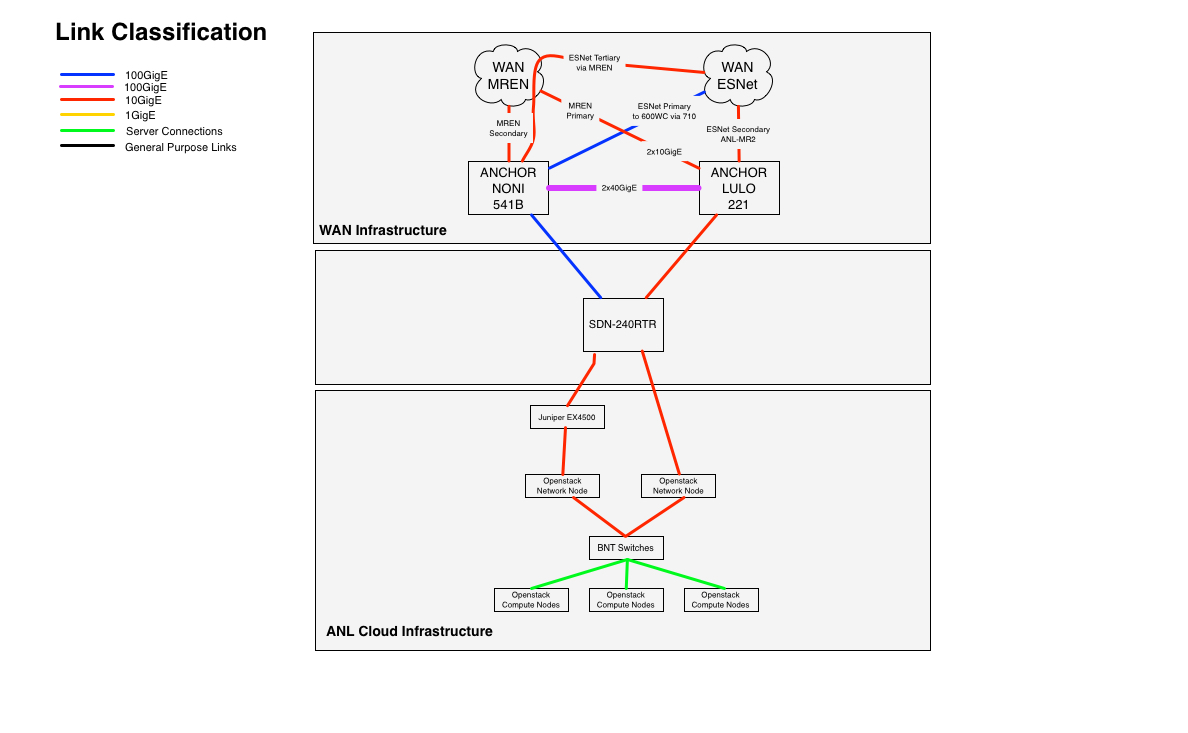
\includegraphics[width=5in]{anl-cloud.jpg}  
\caption{Connectivity for KBase systems at Argonne National Lab.}
\label{kbase:anl} 
\end{center}
\end{figure}


\section{Collaborators}
%Please list facilities, significant users/collaborators, and/or virtual organizations (VOs) that are critical to your work.  A rough estimate on the breadth and depth of the collaboration space (i.e., number of users, number of participating facilities, etc.) is also useful.  Please list geographical endpoints for collaborators.

The KBase project has members from Four National Labs and a number of Universities.   They include:
Argonne National Lab; Brookhaven National Lab; Cold Spring Harbor Lab; Hope College; 
Lawrence Berkeley National Lab; and Oak Ridge National Lab.
Users of the system span the nation and the globe.  

An important partner facility is the Joint Genome Institute (JGI) (see section \ref{sec:kbase-rsa}).  User can use the JGI portal to request data sets to be directly uploaded from JGI into KBase.  JGI resources are located in the NERSC computing facility which the Berkeley resources are also housed.
Work is underway to provide similar mechanisms for data generated by the Environmental Molecular Sciences Laboratory (EMSL) at Pacific Northwest National Lab.

\section{Instruments and Facilities}
%In terms of the present (within 0-2 years), next 2-5 years (beyond the current fiscal year’s budget cycle) and future (beyond 5 years), please describe the network, compute, instruments, and storage resources used for your work. If you are a facility, please describe the resources you make available to your users, or that users deploy at your facility.

KBase has three classes of resources it makes use of for its services and analysis.  They include dedicated hardware (purchased via KBase), the Argonne private cloud (Magellan), and the allocated ASCR compute facilities at ALCF, OLCF, and NERSC.  

%KBase uses several systems distributed across the various sites. At Argonne, KBase uses 
%the Magellan system. At LBNL/National Energy Research Scientific Computing Center (NERSC), KBase has an allocation on Carver. The Kandinsky system at ORNL will be used 
%for data-intensive workloads. 
%KBase plans to run workloads using Mira at Argonne and Cori Phase1 at NERSC. KBase partners with 
%the Joint Genome Institute (JGI), which will result in large-scale ingestion of JGI
%-produced sequence data to provide novel KBase analysis and modeling 
%of these data sets.
\begin{itemize}
\item Present

Table \ref{table:kbase-resources} summarizes the computational and storage resources currently used by KBase.  The network connectivity for the dedicated services is described in the previous section.

\begin{table}[htdp]
\caption{Current KBase Resources}
\begin{center}
\begin{tabular}{| l | c | c | c |}
\hline
 & Cores & Memory & Storage \\ \hline
Dedicated Servers & 492  & 4TB & 424TB \\
Argonne Cloud Allocation & 1756 & 5TB & 60TB \\
HPC Allocations & 2M core hours & & \\ \hline
\end{tabular}
\end{center}
\label{table:kbase-resources}
\end{table}

\item Next 2-5 years

KBase allocates a portion of its budget to maintain and refresh the dedicated hardware.  Based on that allocation we expect the dedicated hardware to scale to roughly 3500 cores and 1.5 PB by 2020.  In this time-frame we would expect that the connectivity for KBase would be upgraded to at least 40Gb or 100Gb based on ingest rates.

\item Beyond 5 years

KBase is an SFA on a 3-year cycle.  The plans beyond five years are currently not defined.  However, if the SFA were to continue, it is likely that KBase would continue to maintain and refresh its server and storage hardware to support continued growth.

\end{itemize}

\section{Process of Science}
%Please describe the way in which the instruments and facilities (as discussed above) are used for knowledge discovery.  Examples might include workflows, data analysis, data reduction, integration of experimental data with simulation data, and so on. The goal is to capture the way in which the instruments and facilities are used (and will be used in the foreseeable future), so we can understand the potential impact of these processes on the network.  If you are a facility, please describe the common use models of your users, with a data-centric or network-centric focus. Please describe this process in terms of:
The KBase project is building novel analysis and modeling techniques for biological data, 
focusing on microbes, plants, and microbial communities, as well as a 
service-oriented architecture that delivers analysis and modeling services to users. Users either upload 
their own data sets or make use of data sets already loaded into KBase, and apply KBase 
operations to these data sets.  Developers can also develop new analysis and modeling approaches and integrate them 
into KBase. The goal here is to provide a common infrastructure for 
large-scale biological data analysis and model creation and refinement. Improvements developed 
through these processes will be rolled out for KBase users over time.

\begin{itemize}
\item Present
At present KBase primarily supports the assembly, annotation and modeling of Microbial data.  It has minimal support for Eukaryotes and microbial communities.  KBase is currently working on enhancements that should improve support for Eukaryotes over the next year.  Improved support for microbial communities should follow after that.  KBase is also working on improvements that will lower the barrier for 3rd party developers to contribute methods and improvements.  This should help to further expand the capabilities of the system and the types of analysis that KBase users can perform in the system.

\item Next 2-5 years
In addition to genomic data, KBase plans to add additional data types in the future.  This could include mass spec data and imaging data.

\item Beyond 5 years

KBase is an BER Science Focus Area (SFA ) on a 3-year funding cycle.  The plans beyond five years are currently not defined.

\end{itemize}

\section{Remote Science Activities}
\label{sec:kbase-rsa}
%Please include a description of any remote instruments or collaborations, and describe how this work does or may have an impact on your network traffic—any connections to major scientific instruments outside of your local instruments and facilities (i.e., supercomputers, particle accelerators, tokamaks, genome sequencers, satellite data…)?

Since KBase is a web-based science platform, all of its users are remote.  Users primarily interact with the system through a "Narrative Interface".  This interface is based on the popular IPython/Jupyter platform with significant customizations done by KBase.  User can upload  data into the system through this interface, conduct analysis, and download analyzed data.  Uploaded datasets can vary significantly in size and quantity.  Currently, users typically upload microbial data sets on the order 100 megabytes in size.  Eukaryotic organisms (plants and fungi) can be significantly larger, 10-100 GBs.  Metagenomc datasets can be even larger exceeding 1 Terabytes in some cases.  The platform currently lacks strong support for these larger datasets, but the project plans to improve support in the coming year for Eukaryotes and following year for Metagenomes.  In addition to genetic data, KBase will be adding support for expression related data such as RNA in the near future.  These datasets can also be large in size (10-100 GBs).

In addition, to user uploaded data, KBase supports direct importing of data from JGI and NCBI (public data sets).  Support is currently limited to isolate microbes, but the project plans to expand support to other data sets.

Finally, KBase has allocations or access to Director's allocations with the ASCR computing facilities.  To date  KBase hasn't made heavy use of these resources, but has efforts to run large-scale pre-computing jobs, assemblies, and other specialized jobs.  This could lead to more flow between KBase systems and the center.  However, the KBase hardware is collocated at ALCF at Argonne and NERSC at Berkeley, so their may be little impact on ESnet.

\section{Software Infrastructure}
%Describe the software used in daily activities of the scientific process.  Please include tools that are used to locally or remotely manage data resources, facilitate the transfer of data sets from or to remote collaborators, or process the raw results into final and intermediate formats.
\begin{figure}[htbp]
\begin{center}
\includegraphics[width=5in]{kbase_roadmap.png}  
\caption{The KBase Roadmap through 2020}
\label{kbase:roadmap} 
\end{center}
\end{figure}

KBase is a essentially a software development project.  Figure \ref{kbase:roadmap} shows the KBase roadmap.  This summarizes the major plans for the KBase platform over the next 4.5 years.  In addition, to the core KBase platform (e.g. data services, job execution services, Narrative and UI components) KBase contains various Science Services that include both JSON-RPC services as well as asynchronous analysis jobs that execute on backend resources (both dedicated and leveraged).

\begin{itemize}
\item Present
KBase operates several data systems to store reference data and user data.  KBase uses a mix of off-the-shelf data stores like MongoDB as well as custom software like Shock and the KBase Workspace.  Data is primarily transferred via HTTP(S). KBase does operate Globus Online End-points, but this end-points are not useable by KBase users at present.


\item Next 2-5 years

Over the next several years KBase plans to continue to enhance its data stores to meet expected scaling demands.  In addition, KBase will be adding support for bulk data uploads.  This will likely lead to an increase in data ingest.  Finally, the roadmap includes plans for new data types and analysis which will drive data ingest.

\item Beyond 5 years

KBase is an SFA on a 3-year cycle.  The plans beyond five years are currently not defined.
\end{itemize}

\section{Cloud Services}
%Please describe current or planned use of cloud services for data analysis, data storage, computing, or other purposes.  Please also include the projected growth in the use of these services.  Note that “cloud” in this case could include commercial clouds such as Amazon, Google, IBM, and Microsoft, or private clouds hosted by some other organization.  Our intent is to understand the ways in which science collaborations are adopting or planning to adopt cloud services so that ESnet can adapt to those changes.

KBase does not currently make use of any commercial cloud services with the exception of standard cloud-based software tools (such as Github, Docker, and Slack).  
KBase currently uses the private Magellan Cloud at Argonne.  It is possible that in the future KBase may utilize public clouds for handling certain burst activities, but doesn't have any specific plans to do so at this time.

\section{Outstanding Issues}
%Please use this space to address or discuss any challenges, barriers, or concerns that should be addressed that have not been asked for. In particular, if there are current network or data transfer performance problems that impact scientific productivity, please describe them.

Most of the current limitations with KBase that relate to networking are due to known constrains in the KBase software.  This includes limits on the ability to upload large data sets, bulk uploads, etc.   The KBase roadmap includes plans for improvements in many of these areas.  
As these limitations and constraints are lifted, KBase may encounter new challenges.  But the network is not currently imposing any serious barriers on KBase.

One important aspect for KBase which is worth noting is around reliability and accessibility.  Through improved replication KBase hopes to move towards a model where the platform is nearly always available.  This could eventually lead to new requirements from the networking layer to allow for seamless load balancing and fail-over between sites.  This may include eventually leveraging software defined networking capabilities between the sites.

\end{document}
